\label{app:gbb-unfolding:optimization}
We use four iterations and the binning is determined by the background subtraction procedure and not by the diagonality of the response matrix (from that point of view, we could go finer).  Figure~\ref{fig:gbb-iterations} shows the dependence of the uncertainty on the number of iterations.  In some cases, the uncertainty could be smaller by using fewer than four iterations; in all cases, there is nothing to gain from going above four iterations.

 % We could go for finer bins based on the response matrix so that should be okay.  The number of iterations can be checked once all of the uncertainties are in place (though we do not expect a big change from four, which is rather standard for the IB method).


\begin{figure}[htpb!]
\begin{center}
  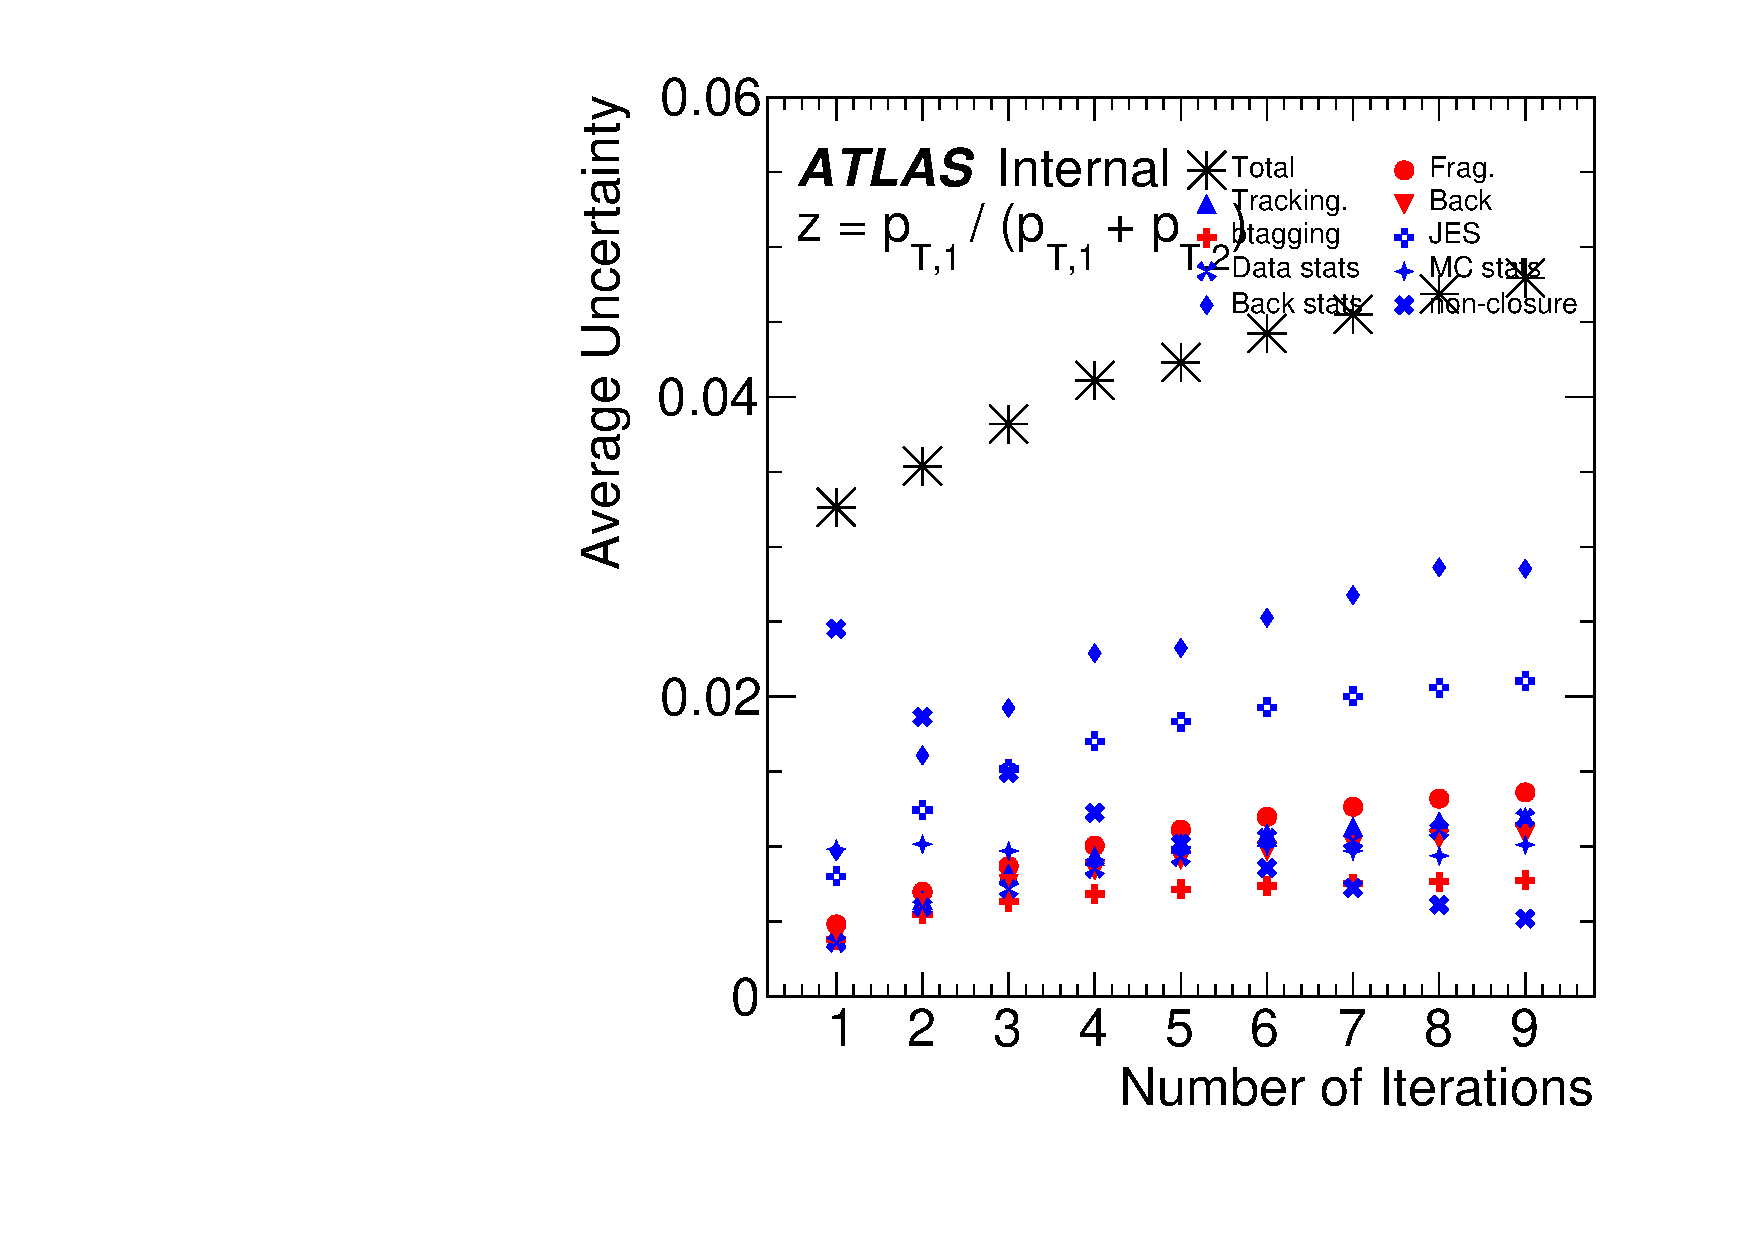
\includegraphics[width=0.45\linewidth]{figures/gbb/Unfolding/IterationsTest_ZpT}
  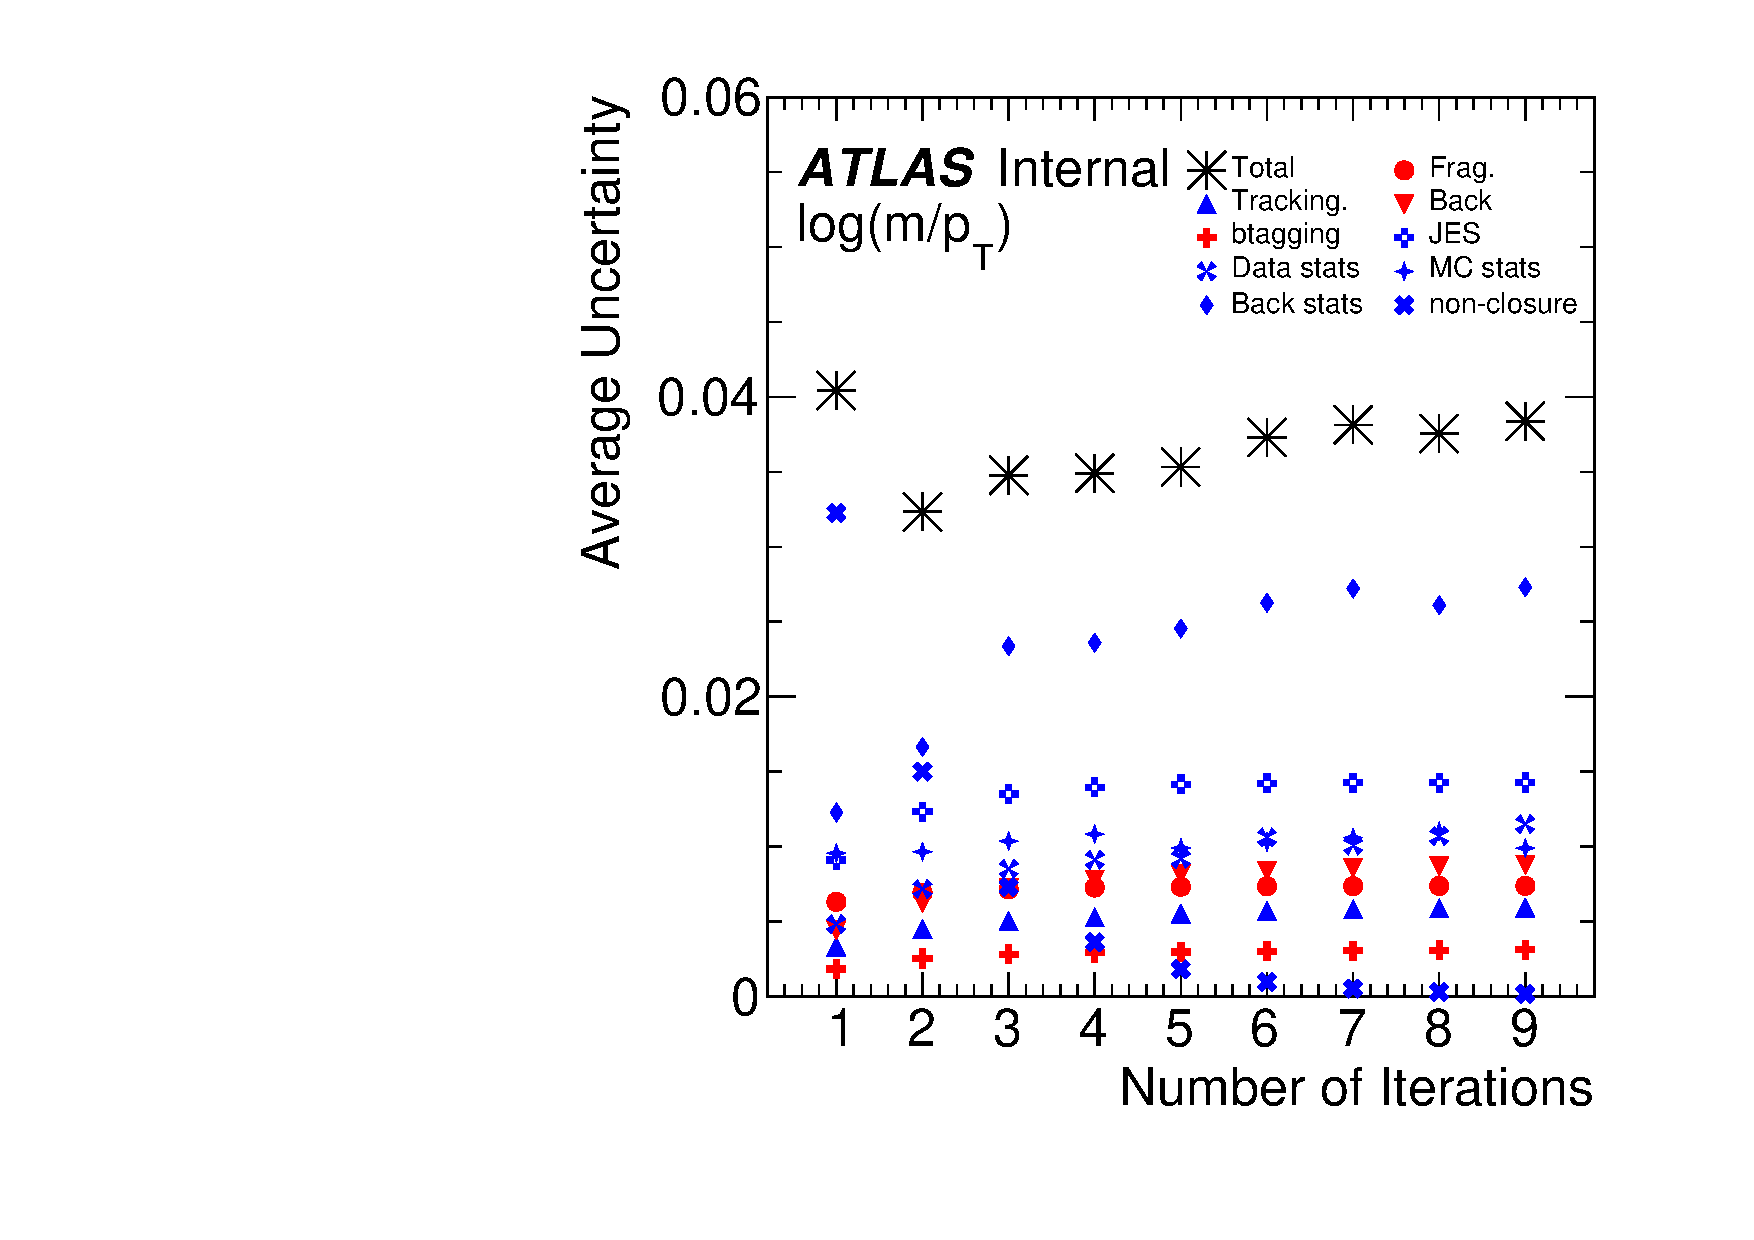
\includegraphics[width=0.45\linewidth]{figures/gbb/Unfolding/IterationsTest_fracmasspt}
  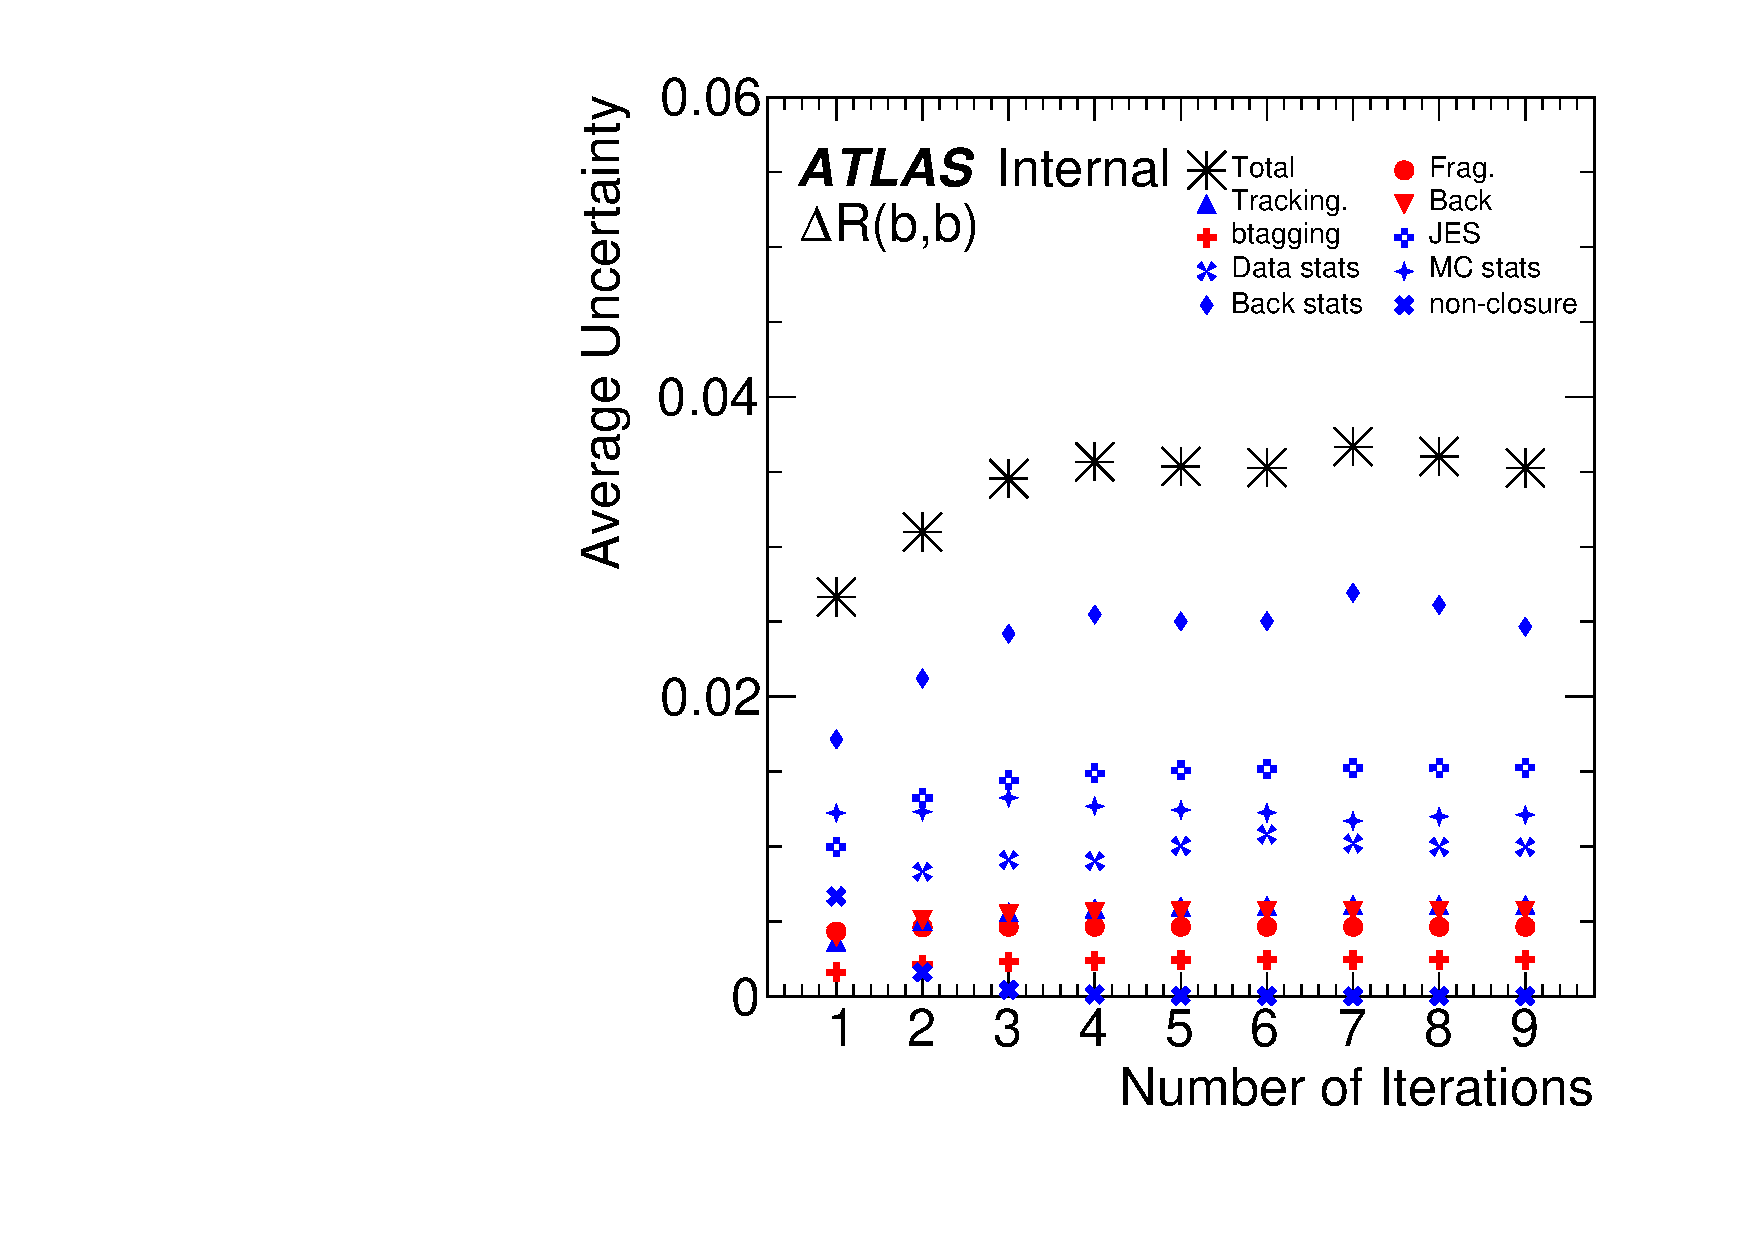
\includegraphics[width=0.45\linewidth]{figures/gbb/Unfolding/IterationsTest_dR}
  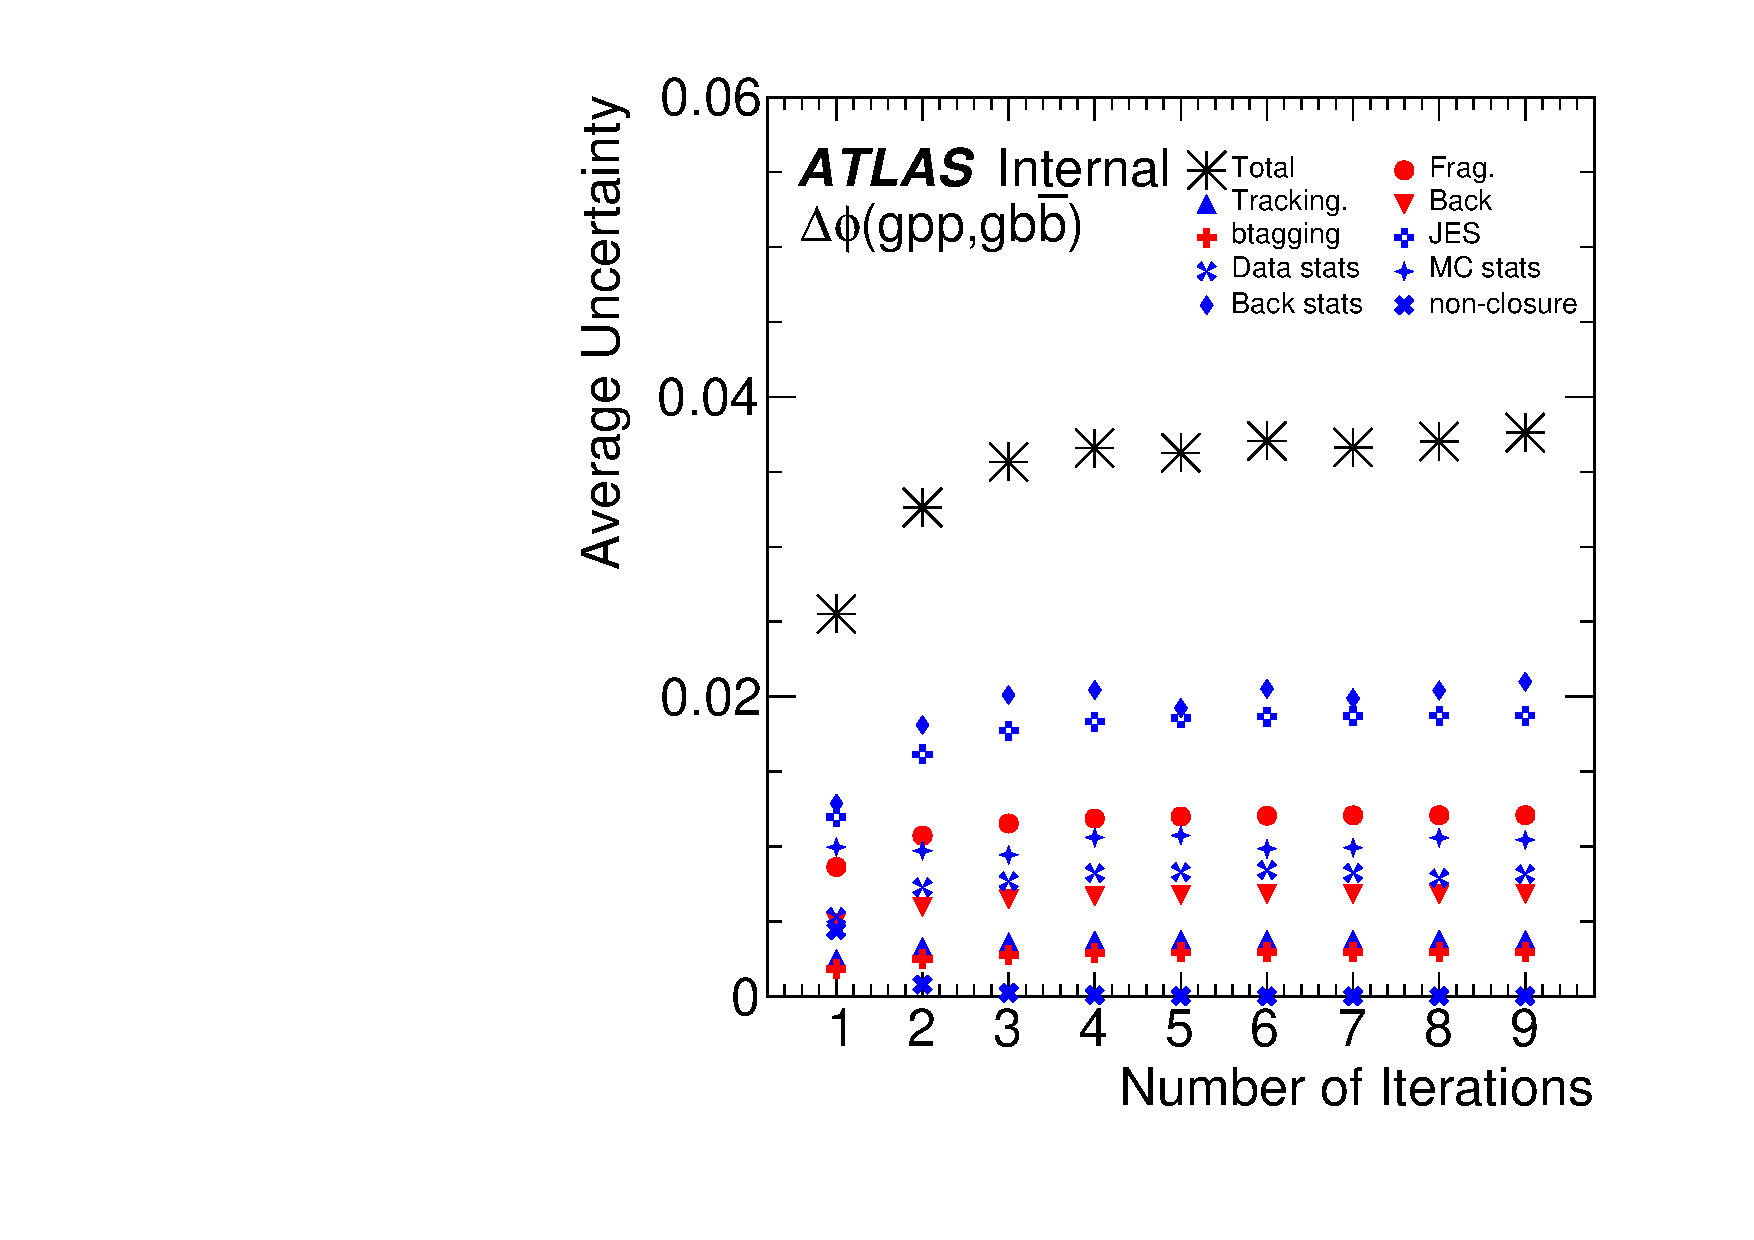
\includegraphics[width=0.45\linewidth]{figures/gbb/Unfolding/IterationsTest_dphi}
\caption[]{The uncertainty as a function of the number of iterations.  See Sec.~\ref{sec:gbb-systs} for a description of the uncertainties. } 
\label{fig:gbb-iterations}
\end{center}
\end{figure}



